\documentclass[a4paper,10pt,oneside]{article}
\usepackage{epsfig}
\usepackage{color}
\usepackage{url}
\usepackage[utf8]{inputenc}
\usepackage[T1]{fontenc}
\usepackage{amsmath}
\usepackage{amssymb}
\usepackage{import}
\usepackage{listings}
\usepackage{color}
\usepackage{textcomp}
\usepackage{upquote}

\definecolor{listinggray}{gray}{0.9}
\definecolor{lbcolor}{rgb}{0.9,0.9,0.9}
\lstset{
%	backgroundcolor=\color{lbcolor},
	tabsize=2,
	rulecolor=,
	language=java,
        basicstyle=\small\ttfamily,
        basewidth=0.51em,
        upquote=true,
        aboveskip={1.5\baselineskip},
        columns=fixed,
        showstringspaces=false,
        extendedchars=true,
        breaklines=true,
%        prebreak =\raisebox{0ex}[0ex][0ex]{\ensuremath{\hookleftarrow}},
 %       frame=single,
        showtabs=false,
        showspaces=false,
        showstringspaces=false,
        identifierstyle=\ttfamily,
%        keywordstyle=\color[rgb]{0,0,1},
%        commentstyle=\color[rgb]{0.133,0.545,0.133},
%        stringstyle=\color[rgb]{0.627,0.126,0.941},
}


\newcommand{\myscale}{0.74}
\newcommand{\vect}[1]{\boldsymbol{#1}}
\newcommand{\code}[1]{\texttt{#1}}

\setlength{\hoffset}{-1in} %left margin will be 0, as hoffset is by default 1inch
\setlength{\voffset}{-1in} %analogous voffset
\setlength{\oddsidemargin}{1.5cm}
\setlength{\evensidemargin}{1.5cm}
\setlength{\topmargin}{1.5cm}
\setlength{\textheight}{26cm}
\setlength{\textwidth}{18cm}




\def\mftitle{jInfer Architecture}
\def\mfauthor{Michal Klempa, Mário Mikula, Robert Smetana, Michal Švirec, Matej Vitásek}
\def\mfadvisor{RNDr. Irena Mlýnková, Ph.D., Martin Nečaský, Ph.D.}
\def\mfplacedate{Praha, 2011}
\title{\bf\mftitle}
\author{\mfauthor \\ Advisors: \mfadvisor}
\date{\mfplacedate}

\ifx\pdfoutput\undefined\relax\else\pdfinfo{ /Title (\mftitle) /Author (\mfauthor) /Creator (PDFLaTeX) } \fi

\begin{document}
\maketitle
Target audience: developers willing to extend jInfer.\\

\textit{Note: we use the term \textbf{inference} for the act of creation of schema throughout this and other jInfer documents.}\\

The description of jInfer architecture will commence by describing the data
structures, namely representations of regular expressions and XML elements,
attributes and simple data.

Afterwards the interfaces of basic inference modules - Initial Grammar Gen-
erator, Simplifier and Schema Generator - will be explained.

Finally, the process of inference will be described.

\section{Package naming conventions}
All packages start with \code{cz.cuni.mff.ksi.jinfer}. Afterwards is the short, normalized name of the module (e.g. \code{base}) and finally the package structure in this module (e.g. \texttt{objects.utils}). All in all, a package in the Base module could look like 
\code{cz.cuni.mff.ksi.jinfer.base.objects.utils}

\section{Data structures}
\subsection{Regular expressions}

For general information on regular expressions, please refer to \cite{wikiregexp}, \cite{automatatheory}.
All classes pertaining to regular expressions can be found in the package \code{cz.cuni.mff.ksi.jinfer.base.regexp}.
In jInfer, we use extended regular expressions as they give us nicer syntax (and easier programming).

Regular expression is implemented as class \code{Regexp} with supplementing classes \code{RegexpInterval} and \code{RegexpType}.
Each \code{Regexp} instance has one of the enum \code{RegexpType} type:
\begin{itemize}
	\item Lambda - empty string (also called $\epsilon$ in literature),
	\item Token - a letter of the alphabet,
	\item Concatenation - one or more regular expression in an ordered sequence. Eg. $(a, b, c, d)$,
	\item Alternation - a choice between one or more regular expressions. Eg. $(a | b | c | d)$,
	\item Permutation - shortcut for all possible permutations of regular expressions. Our syntax to write down permutation is $(a\& b\& c\& d)$.
\end{itemize}

Type of regexp is held in \code{type} member in class \code{Regexp} and can be tested by calling methods \code{isLambda()}, \code{isToken()} etc.

Each \code{Regexp} instance has one instance of \code{RegexpInterval} as member.
Class \code{RegexpInterval} represents POSIX-like intervals for expression:
\begin{itemize}
	\item $a\{m,n\}$ means $a$ at least $m$-times, at most $n$-times,
	\item $a\{m,\}$ means at least $m$-times (unbounded).
\end{itemize}
Interval is either bounded (you have to set both lower and upper bound integers), or unbounded (you have to set only lower bound).
Testing interval commonly follows routine:
\begin{lstlisting}
	RegexpInterval i = r.getInterval();
	if (i.isUnbounded()) {
		print(i.getMin());
	} else {
		print(i.getMin(), i.getMax());
	}
\end{lstlisting}
That is, first check interval for being unbounded, only if it is bounded, you can ask for maximum.

Class \code{Regexp} can represent regular expression over any alphabet.
This is done by using java generics, \code{Regexp} is implemented as \code{Regexp<T>}.
Only token regexps hold instance of type \code{T} in member \code{content}.

Regular expression is in fact $n$-ary tree, for example expression $(a, b, ((c | d), e), f)$ can be viewed as in figure \ref{reg:tree}.
\begin{figure}
\caption{Example tree for regular expression $(a, b, ((c | d), e), f)$} \label{reg:tree}
\centering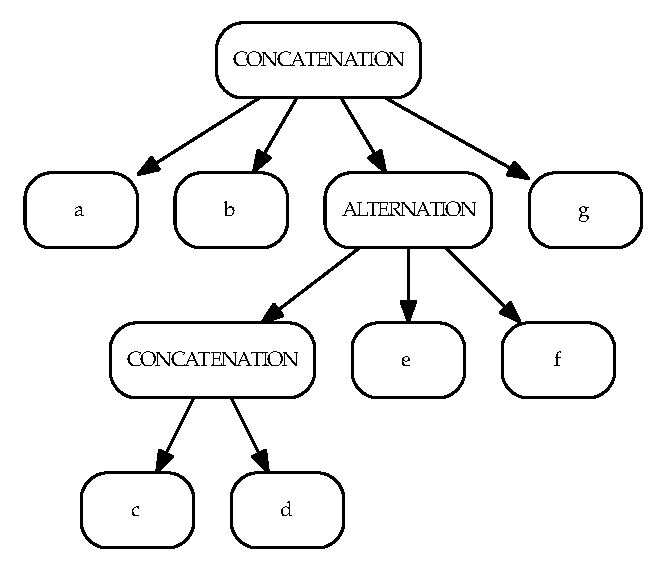
\includegraphics[scale=0.5]{reg_tree.eps}
\end{figure}
We implement this tree by member of \code{Regexp} class called \code{children}, which is of type \code{List<Regexp<T>>}.
List contains children of regexp in means of regexp tree.

Regexp has to obey constraits:
\begin{itemize}
	\item type, children and interval have to be non-null references,
	\item when type is lamba, content and interval has to be null,
	\item when type is token, content has to be non-null,
	\item when type concatenation, alternation or permutation, content has to be null.
\end{itemize}
These constraits are checked by constructors, so the best way to construct new regexps is by using 
methods \code{getToken(), getConcatenation()} etc.

Regexp instance is by default created as immutable, that is, once instantiated, you cannot add more children to list of children, cannot change type, content etc. It is to prevent missuse. In special circumstances, one does not know future children of regexp in time of creation. This occurs mainly in input modules, where by parsing XML data sequentially, one does not know contents of element in time of handling start element event.
For these cases, special \code{getMutable()} method is implemented to obtain regexp with none of members set. One has to fill in all properties carefully and call \code{setImmutable()} aftewards. Proper usage should be one of following:
\begin{lstlisting}
	Regexp<T> r = Regexp.<T>getMutable();
	r.setInterval(...);
	r.setType(RegexpType.LAMBDA);
	r.setImmutable();
\end{lstlisting}
\begin{lstlisting}
	Regexp<T> r = Regexp.<T>getMutable();
	r.setInterval(...);
	r.setType(RegexpType.TOKEN);
	r.setContent(...)
	r.setImmutable();
\end{lstlisting}
\begin{lstlisting}
	Regexp<T> r = Regexp.<T>getMutable();
	r.setInterval(...);
	r.setType(RegexpType.CONCATENATION);
	r.addChild(...);
	r.addChild(...);
	r.addChild(...);
	r.setImmutable();
\end{lstlisting}
	

Finally, regexp contain one useful method for obtaining all leaves in the regexp tree, it is called \code{getTokens()} and it recursively traverses tree returning list of leaves (token type regexps).

\subsection{XML representation}

\nocite{*}
\bibliographystyle{alpha}
\bibliography{literature}

\end{document}
